% Preamble
% ---
\documentclass{article}

% Packages
% ---
\usepackage{amsmath} % Advanced math typesetting
\usepackage[utf8]{inputenc} % Unicode support (Umlauts etc.)
\usepackage[ngerman]{babel} % Change hyphenation rules
\usepackage{hyperref} % Add a link to your document
\usepackage{graphicx} % Add pictures to your document
\usepackage{listings} % Source code formatting and highlighting
\usepackage{booktabs}

\renewcommand{\figurename}{Figure}
%\usepackage[labelsep=endash]{caption}

\usepackage{xcolor}
\lstset { %
    language=C++,
    backgroundcolor=\color{black!5}, % set backgroundcolor
    basicstyle=\footnotesize,% basic font setting
}



\title{%
	MA226 : Monte-Carlo Simulation\\
	 Continuous Random Number Generation\\
	 \large Assignment 4}

\date{09-02-2017}

\author{%
	Turkhade Hrushikesh Pramod\\
	150123044	}	

\begin{document}

	\maketitle
	\pagenumbering{gobble}
	
	\newpage
	\pagenumbering{arabic}
	
	\section{Problem 1}
	\paragraph{}
		We have to generate exponential random variable using Inverse Transform Method.Let, $f(x)$ be the density function of exponential random variable and $X$ be the exponential random variable.
		\paragraph{}
		$X = f^{-1}(U)$ whare $U$ is a uniform random variable.
		
		
	\subsection{Source code of solution in C++}
		\lstinputlisting[language=c++,firstline=6]{code/que1.cpp}
	
	\subsection{Source code of solution in R}
		\lstinputlisting[language=c++,firstline=1]{code/que1.R}
		
		\pagebreak
		\subsection{Observation}
		\paragraph{}
			Here, we observe that the histogram of the generated sample is quite similar to the density function of the exponential distribution.
			
		\subsection{Histograms for the Generated Distribution}
		\begin{figure}[!hb]
  			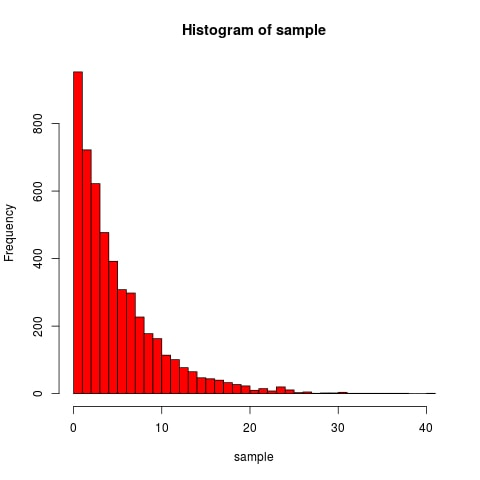
\includegraphics[width=\linewidth]{pic/que1_in_R.jpg}
 			 \caption{Histogram for generated exponential distribution. }
			\label{fig:hist1}
		\end{figure}
		
		\pagebreak
		
		
		\section{Problem 2}
		\paragraph{}
			Now, we have to generate random values from Gamma Random variable. As gamma random variable is sum of $\alpha$ independent exponential random variables of parameter $\lambda$, for $Gamma$ distribution of parameters $(\alpha,\lambda)$.
		\paragraph{}
		Let, $G$ be gamma random variable and $X_i$ be the $i^{th}$ exponential random variable.
		\paragraph{}
		$G = X_1 + X_2 + X_3 + X_4 + X_5$
		
		\subsection{Source code for solution in C++}
		\lstinputlisting[language=c++,firstline=6]{code/que2.cpp}
	
	\subsection{Source code of solution in R}
		\lstinputlisting[language=c++,firstline=1]{code/que2.R}
		
	\pagebreak
		\subsection{Observation}
		\paragraph{}
			Here, we observe that the histogram of the generated sample is quite similar to the density function of the Gamma distribution.
			
		\subsection{Histograms for the Generated Distribution}
		\begin{figure}[!hb]
  			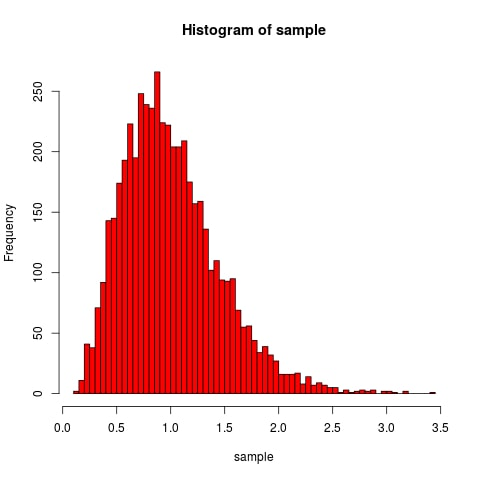
\includegraphics[width=\linewidth]{pic/que2_in_R.jpg}
 			 \caption{Histogram for generated Gamma distribution. }
			\label{fig:hist2}
		\end{figure}
		
		\pagebreak
		
		\section{Problem 3}
		\paragraph{}
		In this we have to use Acceptance-Rejection method to generate samples of a probability distribution given by $f(x)$.
		
		\paragraph{}
		$f(x)=20x(1-x)^3$
		
		\paragraph{}
		Here, we take $g(x)=1$, that is, and $c=2.5$. This satisfies the following condition.

		\paragraph{}
		$ f(x) < c*g(x)$  $ \forall $ $x \in [0,1]$
		
			\subsection{Source code for solution in C++}
		\lstinputlisting[language=c++,firstline=6]{code/que3.cpp}
	
	\subsection{Source code of solution in R}
		\lstinputlisting[language=c++,firstline=1]{code/que3.R}
		
	\pagebreak	 		
			
		\subsection{Histograms for the Generated Distribution}
		\begin{figure}[!hb]
  			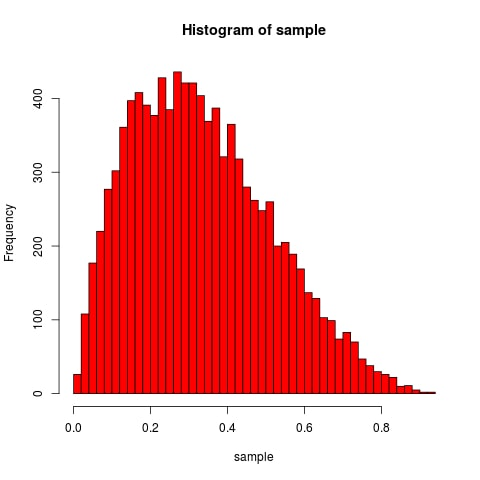
\includegraphics[width=\linewidth]{pic/que3_in_R.jpg}
 			 \caption{Histogram for generated  distribution. }
			\label{fig:hist2}
		\end{figure}
		
		\pagebreak

\end{document}